
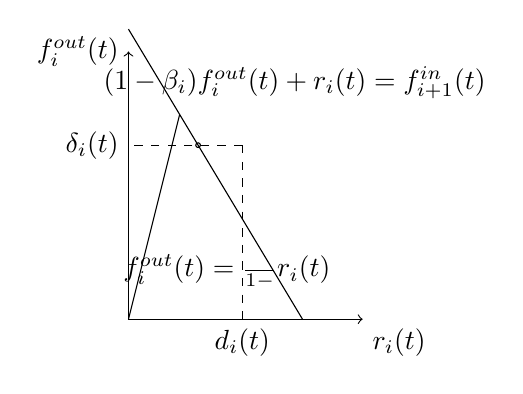
\begin{tikzpicture}[scale=1*.85,domain=0:1]

\def \rampDem{1.7}
\def \dem{2.6}
\def \priorityRat{0.8}
\def \splitRat{0.4}
\def \totalFlow{2.6}
\FontSmall

\coordinate (Z) at (0,0);
\coordinate (I1) at (\rampDem, 0);
\coordinate (I2) at (0, \dem);
\coordinate (I3) at (\rampDem, \dem);

\coordinate (A) at (0, {\totalFlow/(1-\splitRat)});
\coordinate (B) at (\totalFlow, 0);
\coordinate (C) at ({(1-\priorityRat)/\priorityRat*\dem}, \dem);
\coordinate (D) at (intersection of A--B and Z--C);


\draw[->] (Z) -- (3.5,0) node[below right]{$r_i(t)$};
\draw[->] (Z) -- (0,4) node[left]{$f^{\text{out}}_i(t)$};

\draw[dashed] (I3) -- (I1) node[below]{$d_i(t)$};
\draw[dashed] (I3) -- (I2) node[left]{$\delta_i(t)$};


\begin{scope}
%\clip (Z) rectangle (3.5,4);
\draw (A) -- (B) node[yshift=3cm, xshift=-0.1cm]{$(1-\beta_i)f_i^{\text{out}}(t) + r_i(t) = f_{i+1}^{\text{in}}(t)$};
\end{scope}

\draw (Z) -- (D) node[yshift=-2cm, xshift=0.6cm]{$f_i^{\text{out}}(t) = \frac{\priority{\icell}}{1-\priority{\icell}} r_i(t)$};
\draw (intersection of A--B and I3--I2) circle (1pt);

\end{tikzpicture}